\documentclass[12pt,dvipdfmx]{beamer}
\usepackage{pgfpages}
\usepackage{graphicx}
\DeclareGraphicsExtensions{.eps}
\usepackage{listings,jlisting}
\usepackage{fancybox}
\usepackage{hyperref}
\usepackage{multirow}

\newif\ifja
\newif\ifeng
\jafalse
\engtrue

%%%%%%%%%%%%%%%%%%%%%%%%%%%
%%% themes
%%%%%%%%%%%%%%%%%%%%%%%%%%%
\usetheme{Boadilla}
%% no navigation bar
% default boxes Bergen Boadilla Madrid Pittsburgh Rochester
%% tree-like navigation bar
% Antibes JuanLesPins Montpellier
%% toc sidebar
% Berkeley PaloAlto Goettingen Marburg Hannover Berlin Ilmenau Dresden Darmstadt Frankfurt Singapore Szeged
%% Section and Subsection Tables
% Copenhagen Luebeck Malmoe Warsaw

%%%%%%%%%%%%%%%%%%%%%%%%%%%
%%% innerthemes
%%%%%%%%%%%%%%%%%%%%%%%%%%%
% \useinnertheme{circles}	% default circles rectangles rounded inmargin

%%%%%%%%%%%%%%%%%%%%%%%%%%%
%%% outerthemes
%%%%%%%%%%%%%%%%%%%%%%%%%%%
% outertheme
% \useoutertheme{default}	% default infolines miniframes smoothbars sidebar sprit shadow tree smoothtree


%%%%%%%%%%%%%%%%%%%%%%%%%%%
%%% colorthemes
%%%%%%%%%%%%%%%%%%%%%%%%%%%
\usecolortheme{seahorse}
%% special purpose
% default structure sidebartab 
%% complete 
% albatross beetle crane dove fly seagull 
%% inner
% lily orchid rose
%% outer
% whale seahorse dolphin

%%%%%%%%%%%%%%%%%%%%%%%%%%%
%%% fontthemes
%%%%%%%%%%%%%%%%%%%%%%%%%%%
\usefonttheme{serif}  
% default professionalfonts serif structurebold structureitalicserif structuresmallcapsserif

%%%%%%%%%%%%%%%%%%%%%%%%%%%
%%% generally useful beamer settings
%%%%%%%%%%%%%%%%%%%%%%%%%%%
% 
\AtBeginDvi{\special{pdf:tounicode EUC-UCS2}}
% do not show navigation
\setbeamertemplate{navigation symbols}{}
% show page numbers
\setbeamertemplate{footline}[frame number]


%%%%%%%%%%%%%%%%%%%%%%%%%%%
%%% define some colors for convenience
%%%%%%%%%%%%%%%%%%%%%%%%%%%

\newcommand{\mido}[1]{{\color{green}#1}}
\newcommand{\mura}[1]{{\color{purple}#1}}
\newcommand{\ore}[1]{{\color{orange}#1}}
\newcommand{\ao}[1]{{\color{blue}#1}}
\newcommand{\aka}[1]{{\color{red}#1}}

\setbeamercolor{ex}{bg=cyan!20!white}

%%%%%%%%%%%%%%%%%%%%%%%%%%%
%%% how to typset code
%%%%%%%%%%%%%%%%%%%%%%%%%%%

\lstset{language = C,
numbers = left,
numberstyle = {\tiny \emph},
numbersep = 10pt,
breaklines = true,
breakindent = 40pt,
frame = tlRB,
frameround = ffft,
framesep = 3pt,
rulesep = 1pt,
rulecolor = {\color{blue}},
rulesepcolor = {\color{blue}},
flexiblecolumns = true,
keepspaces = true,
basicstyle = \ttfamily\scriptsize,
identifierstyle = ,
commentstyle = ,
stringstyle = ,
showstringspaces = false,
tabsize = 4,
escapechar=\@,
}

\title{Programming Languages (5) \\
  Memory Management}
\institute{}
\author{Kenjiro Taura}
\date{}

\AtBeginSection[] % Do nothing for \section*
{
\begin{frame}
\frametitle{Contents}
\tableofcontents[currentsection,currentsubsection]
\end{frame}
}

\begin{document}
\maketitle

%%%%%%%%%%%%%%%%%%%%%%%%%%%%%%%%%%
\begin{frame}
\ifja
\frametitle{目次}
\fi
\ifeng
\frametitle{Contents}
\fi
\tableofcontents
\end{frame}

%%%%%%%%%%%%%%%%%%%%%%%%%%%%%%%%%%
\ifja
\section{序論}
\fi
\ifeng
\section{Introduction}
\fi
%%%%%%%%%%%%%%%%%%%%%%%%%%%%%%%%%%


%%%%%%%%%%%
\ifja
\begin{frame}
  \frametitle{プログラミング言語のメモリ管理}
\end{frame}
\fi
%%% ENG %%%
\ifeng
\begin{frame}
  \frametitle{Memory management in programming languages}
  \begin{itemize}
  \item all data 
    (integers, floating point numbers, strings, arrays, structs, \ldots)
    used in a program need a space (register or memory) to hold them
  \item ideally, programming languages \ao{\it manage} them on behalf of the programmer;
    i.e.,
    \begin{itemize}
    \item when creating a new object, find an available space
    \item \ao{\it retain} the space as long as the object is still in use
    \item \ao{\it reclaim/reuse} the space when the object is no longer used
    \end{itemize}

  \item three approaches covered

    \begin{center}
      {\scriptsize
    \begin{tabular}{|ll|l|}\hline
      manual        &            & C, C++ \\\hline
      \multirow{2}{*}{garbage collection} & traversing & \multirow{2}{*}{Python, Java, Julia, Go, OCaml, etc.}  \\
                              & reference counting & \\\hline
      Rust ownership          &            & Rust \\\hline
    \end{tabular}}
    \end{center}
    
  \end{itemize}
\end{frame}
\fi
%%%%%%%%%%%

%%%%%%%%%%%%%%%%%%%%%%%%%%%%%%%%%% 
\ifja
\section{C/C++のメモリ管理}
\fi
\ifeng
\section{Manual Memory Management in C/C++}
\fi
%%%%%%%%%%%%%%%%%%%%%%%%%%%%%%%%%% 

%%%%%%%%%%%%%%%%%%%%%%%%%%%%%%%%%%
\ifja
\begin{frame}[fragile]
\frametitle{動機づけ: C/C++言語のメモリ割り当て}
\begin{enumerate}
\item \ao{大域変数/配列}
\item \aka{局所変数/配列}
\item \ore{ヒープ}
\begin{lstlisting}
@\ao{\tt int g; int ga[10];}@
int foo() {
  @\aka{\tt int l; int la[10];}@
  int * a = &g;
  int * b = ga;
  int * c = &l;
  int * d = la;
  int * e = @\ore{\tt malloc(sizeof(int));}@ 
}
\end{lstlisting}
\item 寿命(lifetime)
\begin{tabular}{|l|l|l|}\hline
      & 開始 & 終了 \\\hline
大域  & プログラム開始時 & プログラム終了時 \\
局所  & ブロック開始時 & ブロック終了時 \\
ヒープ & malloc, new & free, delete \\\hline
\end{tabular}

\item 注: 以降の議論では「変数」も「配列」も合わせて変数と呼ぶ
  (両者の区別は重要ではない)
\end{enumerate}
\end{frame}
\fi
%%% ENG %%%
\ifeng
\begin{frame}[fragile]
  \frametitle{Memory allocation in C/C++}

  \begin{columns}
    \begin{column}{0.5\textwidth}
\begin{enumerate}
\item \ao{Global variables/arrays}
\item \aka{Local variables/arrays}
\item \ore{Heap}
\end{enumerate}
\end{column}    
\begin{column}{0.5\textwidth}
\begin{lstlisting}
@\ao{\tt int g; int ga[10];}@
int foo() {
  @\aka{\tt int l; int la[10];}@
  int * a = &g;
  int * b = ga;
  int * c = &l;
  int * d = la;
  int * e = @\ore{\tt malloc(sizeof(int));}@ 
}
\end{lstlisting}
\end{column}
\end{columns}

\begin{itemize}
\item lifetime
\begin{tabular}{|l|l|l|}\hline
            & starts        & ends \\\hline
\ao{global} & when the program starts & when program ends \\
\aka{local} & when a block starts & when a block ends \\
\ore{heap}  & malloc, new & free, delete \\\hline
\end{tabular}

\item note: the following discussion
  calls all of them {\it objects}
\end{itemize}
\end{frame}
\fi

%%%%%%%%%%%%%%%%%%%%%%%%%%%%%%%%%%

\ifja
\begin{frame}[fragile]
\frametitle{あ}
\begin{itemize}
\item あ
\end{itemize}
\begin{lstlisting}
あ
\end{lstlisting}
\end{frame}
\fi
%%% ENG %%%
\ifeng
\begin{frame}[fragile]
  \frametitle{What could go wrong in manual memory management (e.g., C/C++)?}
  \begin{itemize}
  \item heap-allocated (i.e., {\tt new}/{\tt malloc}'ed) memory
    must be {\tt delete}/{\tt free}d at the right spot
    \begin{itemize}
    \item
      \ao{\it premature free} $=$
      using it after {\tt delete/free} $\rightarrow$ memory corruption
\begin{lstlisting}
node * foo() {
  node * m = @\aka{\tt new node("Mimura")}@;
  node * o = m;
  delete m;
  ... o->name ...
}    
\end{lstlisting}
      
    \item \ao{\it memory leak} $=$
      not {\tt delete/free}ing no-longer-used memory $\rightarrow$
      (eventually) out of memory
      
\begin{lstlisting}
node * foo() {
  node * m = @\aka{\tt new node("Mimura")}@;
  node * o = new node("Ohtake");
  return o;
}    
\end{lstlisting}
    \end{itemize}
\end{itemize}
\end{frame}


\begin{frame}[fragile]
  \frametitle{What could go wrong in manual memory management (e.g., C/C++)?}
  \begin{itemize}
  \item stack-allocated memory are automatically reclaimed when
    it goes out of scope
    \begin{itemize}
    \item using it afterwards $\equiv$ premature delete
    \end{itemize}
\begin{lstlisting}
node * foo() {
  node m = node("Mimura");
  node o = @\aka{\tt node("Ohtake")}@;
  return @\aka{\tt \&o}@;
}    
\end{lstlisting}
\begin{lstlisting}
node * foo() {
  node   m =     @\aka{\tt node("Mimura")}@;
  node * o = new node("Ohtake");
  o->friend = @\aka{\tt \&m}@;
  return o;
}    
\end{lstlisting}
  \end{itemize}
  

\end{frame}


\begin{frame}
  \frametitle{Tools to make C/C++ memory management safer}
  \begin{itemize}
  \item \ao{\tt valgrind} (memory checker)
    \begin{itemize}
    \item detect memory-related errors (use after free, memory leak, out of bound accesses, etc.)
    \end{itemize}
  \item Boehm garbage collection library for C/C++
    \begin{itemize}
    \item automatically garbage-collect memory blocks allocated by malloc/new
    \end{itemize}
  \end{itemize}
\end{frame}
\fi
%%%%%%%%%%%%%%%%%%%%%%%%%%%%%%%%%%


%%%%%%%%%%%%%%%%%%%%%%%%%%%%%%%%%%
\iffalse
\ifja
\begin{frame}[fragile]
\frametitle{起きうる間違い}
\begin{itemize}
\item 寿命を超えて変数をアクセスする
\item ヒープから割り当てた変数を開放し忘れる\ao{(メモリリーク)}
\end{itemize}
\end{frame}
\fi
%%% END %%%
\ifeng
\begin{frame}[fragile]
\frametitle{How they can go wrong}
\begin{itemize}
\item access an object beyond its lifetime 
\item forget to release/reclaim
  an object \ao{(memory leak)}
\end{itemize}
\end{frame}
\fi
\fi

%%%%%%%%%%%%%%%%%%%%%%%%%%%%%%%%%%
\iffalse
\ifja
\begin{frame}[fragile]
\frametitle{寿命を超えたアクセス}
\begin{itemize}
\item 変数の「寿命」の意味: 
  「寿命の間」に限り,変数はまともに振る舞う
  $=$代入した値を覚えておいてくれる.
\item 寿命を超えたアクセス
  \begin{itemize}
  \item 仕様: 「未定義」
  \item 実際の症状: その変数が(寿命の間)置かれていた領域が,
    開放される
    \begin{itemize}
    \item $\Rightarrow$ 他の変数のために再利用される
    \item $\Rightarrow$ \aka{知らぬ間に壊される,他のデータを壊す}
    \item もちろん実行時の型安全性も保証されなくなる
    \end{itemize}
  \end{itemize}
\end{itemize}
\end{frame}
\fi
%%% END %%%
\ifeng
\begin{frame}[fragile]
\frametitle{Accessing an object after its lifetime}
\begin{itemize}
\item what is the ``lifetime'' of an object:
  the period in which it should behave as expected
  ($=$ remembers the assigned value)
\item if you access an object after its lifetime
  \begin{itemize}
  \item specification: ``undefined''
  \item what happens in practice:
    the memory region that hosted the object (during its lifetime)
    may have been released
    \begin{itemize}
    \item $\Rightarrow$ the region may have been reused for other objects
    \item $\Rightarrow$ \aka{writing to the object corrupts
        other objects and vice versa}
    \item type safety will be lost 
    \end{itemize}
  \end{itemize}
\end{itemize}
\end{frame}
\fi
\fi

%%%%%%%%%%%%%%%%%%%%%%%%%%%%%%%%%%
\iffalse
\ifja
\begin{frame}[fragile]
\frametitle{寿命を超えたアクセスの例}
\begin{columns}
\begin{column}{0.05\textwidth}
\end{column}
\begin{column}{0.3\textwidth}
局所変数
\begin{lstlisting}
int * foo() {
  int a[100];
  return a;
}

int main() {
  int * p = foo();
  @\aka{\tt p[0]}@ = @\ldots@
}
\end{lstlisting}
\end{column}
\begin{column}{0.05\textwidth}
\end{column}
\begin{column}{0.5\textwidth}
ヒープ
\begin{lstlisting}
typedef struct list { 
  int val;
  struct list * next;
} list;

void destroy_list(list * n) {
  for (list * p = n; p; p = @\aka{\tt p->}@next) {
    free(p);
  }
}
\end{lstlisting}
\end{column}
\end{columns}
\end{frame}
\fi
%%% END %%%
\ifeng
\begin{frame}[fragile]
\frametitle{An example accessing an object beyond its lifetime}
\begin{columns}
\begin{column}{0.05\textwidth}
\end{column}
\begin{column}{0.3\textwidth}
local variable
\begin{lstlisting}
int * foo() {
  int a[100];
  return a;
}

int main() {
  int * p = foo();
  @\aka{\tt p[0]}@ = @\ldots@
}
\end{lstlisting}
\end{column}
\begin{column}{0.05\textwidth}
\end{column}
\begin{column}{0.5\textwidth}
heap
\begin{lstlisting}
typedef struct { ... } S;

void destroy_list(list * n) {
  S * p = malloc(sizeof(S));
  S * q = p;
  free(p);
  .. @\aka{\tt q->x}@ .. 
}
\end{lstlisting}
\end{column}
\end{columns}
\end{frame}
\fi
\fi
%%%%%%%%%%%%%%%%%%%%%%%%%%%%%%%%%%%%%%%%%%%%%%%%%%%%

%%% ENG %%%
\ifeng
\begin{frame}
  \frametitle{Note : it is not a {\it pointer} that is to blame}
  \begin{itemize}
  \item C/C++ are notriously unsafe languages
  \item a common misconception is
    they are unsafe \aka{\it because they expose pointers} to the programmer
  \item sure, many features that make C/C++ unsafe are related to pointers
    in one way or another,
  \item yet this is a misconception because
    \begin{itemize}
    \item eliminating pointers from the surface of a language does not solve
      the memory management problem, and
    \item languages exposing pointers can be made safe
    \end{itemize}
  \end{itemize}
\end{frame}

%%%%%%%%%%%%%%%%%%%%%%%%%%%%%%%%%%
\section{The Root of the Problem}
%%%%%%%%%%%%%%%%%%%%%%%%%%%%%%%%%%


%%% ENG %%%
\ifeng
\begin{frame}
  \frametitle{Data representation}
  \begin{itemize}
  \item data in your program must be somehow represented in the machine code
  \item some data (e.g., integers and floating point numbers)
    can be trivially mapped to machine representations
  \item less trivial is how to map
    \begin{itemize}
    \item multiword data (structs),
    \item unknown-size or large data (e.g., arrays and strings),
    \item mutable data,
    \item recursive data (lists),
    \item etc.
    \end{itemize}
  \end{itemize}
\end{frame}
\fi

%%%%%%%%%%%%%%%%%%%%%%%%%%%%%%%%%% 
\ifeng
\begin{frame}[fragile]
  \frametitle{Two strategies}
  \begin{itemize}
  \item immediate
    \begin{itemize}
    \item []
      \includegraphics[width=0.8\textwidth]{out/pdf/svg/data_representation_1.pdf}
    \end{itemize}
  \item indirect
    \begin{itemize}
    \item []
      \includegraphics[width=0.8\textwidth]{out/pdf/svg/data_representation_4.pdf}
    \end{itemize}
  \end{itemize}
\end{frame}
\fi


%%%%%%%%%%%%%%%%%%%%%%%%%%%%%%%%%% 
\ifeng
\begin{frame}
  \frametitle{Immediate representation}
  \begin{itemize}
  \item<1-> typically used for small data (integers, floating point numbers, characters, etc.)
    that fit on a single register (e.g., 64 bits)
  \item<2-> upon an assignment-like operation,
    the whole data gets copied (cheap as data are small)
  \end{itemize}

  \begin{center}
    \only<1>{\includegraphics[width=\textwidth]{out/pdf/svg/data_representation_1.pdf}}%
    \only<2>{\includegraphics[width=\textwidth]{out/pdf/svg/data_representation_2.pdf}}%
    \only<3>{\includegraphics[width=\textwidth]{out/pdf/svg/data_representation_3.pdf}}%
  \end{center}

\end{frame}
\fi

%%%%%%%%%%%%%%%%%%%%%%%%%%%%%%%%%% 
\ifeng
\begin{frame}
  \frametitle{Indirect representation}
  \begin{itemize}
  \item<1-> typically used for multi-word data
  \item<2-> upon an assignment-like operation, there are two choices
    \begin{enumerate}
    \item<3-> \ao{(by-value)} copies the whole data, or
    \item<4-> \ao{(by-reference)} copies only the address and
      \ao{\it share} data in memory
    \end{enumerate}
  \end{itemize}

  \begin{center}
    \only<1>{\includegraphics[width=\textwidth]{out/pdf/svg/data_representation_4.pdf}}%
    \only<2>{\includegraphics[width=\textwidth]{out/pdf/svg/data_representation_5.pdf}}%
    \only<3>{\includegraphics[width=\textwidth]{out/pdf/svg/data_representation_6.pdf}}%
    \only<4>{\includegraphics[width=\textwidth]{out/pdf/svg/data_representation_7.pdf}}%
  \end{center}
\end{frame}
\fi

%%%%%%%%%%%%%%%%%%%%%%%%%%%%%%%%%% 
\ifeng
\begin{frame}[fragile]
  \frametitle{By-value vs. by-reference?}
  \begin{itemize}
  \item it affects \ao{\it behavior (semantics) of mutable data}; e.g.,
\begin{lstlisting}
p = Point{x=456, y=789};
q = p;            // by-value or by-reference?
p.x = 1000;
print(q.x)        // 456 or 1000?
\end{lstlisting}
\item therefore, for \ao{\it mutable data, by-reference} is the only choice
\item the choice does not affect the semantics of
  \ao{\it immutable data}, so it is up to implementation
\end{itemize}

\begin{tabular}{c|c}
  \includegraphics[width=0.48\textwidth]{out/pdf/svg/data_representation_6.pdf} 
  & \includegraphics[width=0.48\textwidth]{out/pdf/svg/data_representation_7.pdf} \\
  by-value & by-reference
\end{tabular}

\end{frame}
\fi

%%%%%%%%%%%%%%%%%%%%%%%%%%%%%%%%%% 
\ifeng
\begin{frame}[fragile]
  \frametitle{It is not exposing a pointer that is to blame}
  \begin{itemize}
  \item were there no by-reference data,
    memory management problem would be largely non-existent
    \begin{itemize}
    \item if a variable is gone, the data it points to is gone, too
    \end{itemize}
  \item the difficulty arises as soon as data are \ao{\it shared} (i.e.,
    whose address may be held by multiple locations)
    \begin{itemize}
    \item yet it is essential/unavoidable to implement
      mutable and/or implement large data efficiently, among others
    \end{itemize}
  \end{itemize}

\begin{tabular}{c|c}
  \includegraphics[width=0.48\textwidth]{out/pdf/svg/data_representation_6.pdf} 
  & \includegraphics[width=0.48\textwidth]{out/pdf/svg/data_representation_7.pdf} \\
  by-value & by-reference
\end{tabular}
\end{frame}
\fi

%%%%%%%%%%%%%%%%%%%%%%%%%%%%%%%%%% 
\ifeng
\begin{frame}[fragile]
  \frametitle{The fundamental problem}
  \begin{itemize}
  \item the problem is how to know which memory block can be safely reclaimed/reused
    when
    \begin{itemize}
    \item there may be multiple pointers to a single memory block,
    \item which allow arbitrary graph of memory blocks
    \end{itemize}
  \end{itemize}
  \begin{center}
    \includegraphics[width=0.7\textwidth]{out/pdf/svg/gc_basic_4.pdf}
  \end{center}
\end{frame}

%%%%%%%%%%%%%%%%%%%%%%%%%%%%%%%%%%
\iffalse
\ifja
\begin{frame}[fragile]
\frametitle{図解 (Q2)}

\begin{center}
  \includegraphics[width=\textwidth]{out/pdf/lsvg/mm_quiz_1.pdf}
\end{center}

\end{frame}
\fi
%%% ENG %%%
\ifeng
\begin{frame}[fragile]
\frametitle{Illustration (Q2)}

  \begin{center}
  \includegraphics[width=\textwidth]{out/pdf/lsvg/mm_quiz_1.pdf}
  \end{center}

\end{frame}
\fi
%%%%%%%%%%%%%%%%%%%%%%%%%%%%%%%%%%

%%%%%%%%%%%%%%%%%%%%%%%%%%%%%%%%%%
\ifja
\begin{frame}[fragile]
\frametitle{図解 (Q3)}

\begin{center}
  \includegraphics[width=\textwidth]{out/pdf/lsvg/mm_quiz_2.pdf}
\end{center}

\end{frame}
\fi
%%% ENG %%%
\ifeng
\begin{frame}[fragile]
\frametitle{Illustration (Q3)}

\begin{center}
  \includegraphics[width=\textwidth]{out/pdf/lsvg/mm_quiz_2.pdf}
\end{center}

\end{frame}
\fi
\fi
%%%%%%%%%%%%%%%%%%%%%%%%%%%%%%%%%%

%%%%%%%%%%%%%%%%%%%%%%%%%%%%%%%%%%
\ifja
\section{ガベージコレクション(GC)}
\fi
\ifeng
\section{Garbage Collection (GC) : A Brief Introduction}
\fi
%%%%%%%%%%%%%%%%%%%%%%%%%%%%%%%%%% 
%%%%%%%%%%%%%%%%%%%%%%%%%%%%%%%%%%
\ifja
\begin{frame}
\frametitle{ガベージコレクション(Garbage Collection; GC)}
\begin{itemize}
\item つまりは「寿命」と「アクセスする期間」が一致していないのが問題
  \begin{itemize}
  \item 寿命後でもアクセスできてしまう
  \item もうアクセスしないのに開放しない(生きっ放し)
  \end{itemize}

\item $\Rightarrow$ ガベージコレクション(GC)
  \begin{itemize}
  \item \ao{今後アクセスされ得るものは残し,され得ないものは開放(再利用)}する
  \item それを処理系が自動的に行う
  \item $\Rightarrow$ リークや,寿命後のアクセスによるメモリ破壊をなくす
  \item C, C++, 古代の言語以外はほぼ搭載している
  \end{itemize}
\item \ao{今後アクセスされ\{得る・得ない\}もの}なんてなぜわかるのでしょう?
\end{itemize}
\end{frame}
\fi
%%% END %%%
\ifeng
\begin{frame}
\frametitle{Garbage Collection (GC)}
\begin{itemize}
\item the fundamental problem issue is
  the mismatch between
  \begin{itemize}
  \item the period in which objects are accessed
  \item the period in which the memory block for it is retained
  \end{itemize}

  \begin{center}
    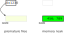
\includegraphics[width=0.4\textwidth]{out/pdf/svg/poitners.pdf}
  \end{center}

\item<2-> $\Rightarrow$ \ao{Garbage collection (GC)}
  \begin{itemize}
  \item \ao{ratain memory block for objects if they could ever be accessed in future
      and reclaim otherwise}
  \item the system automatically does that
  \item $\Rightarrow$ eliminate memory leak and corruption
  \end{itemize}
\item<3-> \ao{the question:} how does the system know
  \ao{\it which objects may be accessed in future}?
\end{itemize}
\end{frame}
\fi

%%%%%%%%%%%%%%%%%%%%%%%%%%%%%%%%%%
\ifja
\begin{frame}[fragile]
\frametitle{今後アクセスされ\{得る・得ない\}もの}
\begin{columns}
\begin{column}{0.6\textwidth}
\begin{itemize}
\item 正確な判定は決定不能
\item ({\tt f(x)}開始時点で)
「{\tt p}が指している領域は今後アクセスされる」
$\iff$
「{\tt f(x)}が終了して0を返す」
$\rightarrow$ 停止問題を解く必要が\ldots

\item $\rightarrow$「今後アクセスされるかも」を大きめに評価
  \begin{itemize}
  \item \aka{NG:} 実はアクセスされるものを回収
  \item \ao{OK:} 実はアクセスされないものを回収しない
  \end{itemize}

\item 上の例ならば{\tt p}はアクセスされる「かも」
($\rightarrow$回収しない)とわかれば十分
\end{itemize}
\end{column}

\begin{column}{0.35\textwidth}
\begin{lstlisting}
int main() {
  if (f(x) == 0) {
    printf("%d\n", p->f->x);
  }    
}
\end{lstlisting}
\begin{center}
%\includegraphics[width=0.6\textwidth]{out/pdf/img/1354150858.pdf}    
\end{center}
\end{column}
\end{columns}
\end{frame}
\fi
%%% END %%%
\ifeng
\begin{frame}[fragile]
\frametitle{Objects that may \{ever/never\} be accessed}
\begin{itemize}
\item the precise judgment is undecidable
\end{itemize}
\begin{columns}
\begin{column}{0.6\textwidth}
\begin{itemize}
\item (at the start of line 2)
``the object pointed to by {\tt p} will ever be accessed''
$\iff$
``{\tt f(x)} will terminate and return 0''
$\rightarrow$ you need to be able to solve the halting problem\ldots
\end{itemize}
\end{column}

\begin{column}{0.35\textwidth}
\begin{lstlisting}
int main() {
  if (f(x) == 0) {
    printf("%d\n", p->f->x);
  }    
}
\end{lstlisting}
\begin{center}
%\includegraphics[width=0.6\textwidth]{out/pdf/img/1354150858.pdf}    
\end{center}
\end{column}
\end{columns}

\begin{itemize}
\item $\rightarrow$ \ao{\it conservatively}
  estimate objects that \ao{\it may be} accessed in future
  \begin{itemize}
  \item \aka{NEVER} reclaim those that are accessed
  \item \ao{OK} not to reclaim those that are in fact never accessed
  \end{itemize}

\item in the above example, OK to retain objects pointed to by {\tt p}
  when the line 2 is about to start
\end{itemize}
\end{frame}
\fi

%%%%%%%%%%%%%%%%%%%%%%%%%%%%%%%%%%
\ifja
\begin{frame}[fragile]
\frametitle{アクセスされる「かも」しれないデータ}
{\small
\begin{itemize}
\item \aka{大域変数}
\item 現在活性な(始まったが終了していない)
  関数呼び出しの\aka{局所変数}
\item<2->\ore{それらからポインタをたどって辿り着くデータ}
\end{itemize}}

\begin{columns}
\begin{column}{0.25\textwidth}
\begin{lstlisting}[]
int * @\aka{\tt s}@;
int * @\aka{\tt t}@;
void h() { ... }
void g() {
  ... 
  h();
  ... = @\aka{\tt p}@->x ...  }
void f() {
  ... 
  g()
  ... = @\aka{\tt q}@->y ... }
int main() {
  ... 
  f()
  ... = @\aka{\tt r}@->z ... }
\end{lstlisting}
\end{column}

\begin{column}{0.65\textwidth}
\begin{center}
\only<1>{\includegraphics[width=\textwidth]{out/pdf/svg/gc_basic_0.pdf}}%
\only<2>{\includegraphics[width=\textwidth]{out/pdf/svg/gc_basic_3.pdf}}
\end{center}
\end{column}
\end{columns}
\end{frame}
\fi
%%% END %%%
\ifeng
\begin{frame}[fragile]
\frametitle{Objects that ``may be'' accessed}
{\small
\begin{itemize}
\item \ao{global variables}
\item \aka{local variables} of
  active function calls (calls that have started but have not finished)
\item<2->\ore{objects reachable from them by traversing pointers}
\end{itemize}}

\begin{columns}
\begin{column}{0.35\textwidth}
  \begin{itemize}
  \item []
\begin{lstlisting}[]
int * @\ao{\tt s}@, * @\ao{\tt t}@;
void h() { ... }
void g() {
  ... 
  h();
  ... = @\aka{\tt p}@->x ...  }
void f() {
  ... 
  g()
  ... = @\aka{\tt q}@->y ... }
int main() {
  ... 
  f()
  ... = @\aka{\tt r}@->z ... }
\end{lstlisting}
\end{itemize}
\end{column}

\begin{column}{0.65\textwidth}
\begin{center}
\only<1>{\includegraphics[width=0.8\textwidth]{out/pdf/svg/gc_basic_0.pdf}}%
\only<2>{\includegraphics[width=0.8\textwidth]{out/pdf/svg/gc_basic_3.pdf}}
\end{center}
\end{column}
\end{columns}
\end{frame}
\fi

%%%%%%%%%%%%%%%%%%%%%%%%%%%%%%%%%%
\ifja
\subsection{基本原理と用語}
\fi
\ifeng
\subsection{Basics and Terminologies}
\fi
%%%%%%%%%%%%%%%%%%%%%%%%%%%%%%%%%% 
%%%%%%%%%%%%%%%%%%%%%%%%%%%%%%%%%%
\ifja
\begin{frame}
\frametitle{GCの基本原理(と用語)}
\begin{itemize}
\item \ao{オブジェクト:} メモリ割り当て・回収の単位(Cならばmalloc)
\item \ao{ルート:}
  大域変数や現在活性中の関数の局所変数など,
  ポインタをひとつもたどらずにアクセスされうるオブジェクト
\item \ao{到達可能(reachable):}
  ポインタをたどってたどりつける
\item \ao{生きている(live),死んでいる(dead):}
  今後アクセスされうる,され得ない
\item \ao{ゴミ:} 死んでいるオブジェクト
\item \ao{collector:} GCをするプログラム(やスレッド/プロセス)
\item \ao{mutator:} 要するにユーザプログラムのこと(vs. collector).
  超GC目線な言葉. ユーザプログラムは「グラフを書き換える(mutateする)人」
\end{itemize}
\begin{columns}
\begin{column}{0.8\textwidth}
\begin{beamercolorbox}{ex}
\vskip0.5cm
GCの基本原理: \\
\ao{ルートから到達不能なオブジェクトは死んでいる}
\vskip0.5cm
\end{beamercolorbox}
\end{column}
\begin{column}{0.2\textwidth}
\begin{center}
%\includegraphics[width=0.8\textwidth]{out/pdf/img/1354150858.pdf}
\end{center}
\end{column}
\end{columns}
\end{frame}
\fi
%%% END %%%
\ifeng
\begin{frame}
\frametitle{The basic workings (and terminologies) of GC}
\begin{itemize}
\item<1-> \ao{an object:} the unit of automatic memory allocation/release
  (malloc in C; objects in Java; etc.)
\item<2-> \ao{the root:}
  objects accessible without traversing pointers, such as
  global variables and local variables of active function calls
\item<3-> \ao{reachable objects:} objects reachable from the root
  by traversing pointers
\item<4-> \ao{live / dead objects:}
  objects that \{may be / never be\} accessed in future 
\item<5-> \ao{garbage:} dead objects
\item<6-> \ao{collector:} the program (or the thread/process) doing GC
\item<7-> \ao{mutator:} the user program (vs. collector).
  very GC-centric terminology, viewing the user program
  as someone simply ``mutating'' the graph of objects
\end{itemize}
\begin{center}
  \begin{columns}
    \begin{column}{0.7\textwidth}
\only<8->{      
\begin{beamercolorbox}{ex}
\vskip0.1cm
the basic principle of GC: \\
\ao{objects unreachable from the root are dead}
\vskip0.1cm
\end{beamercolorbox}}
    \end{column}
  \end{columns}
    \end{center}
\end{frame}
\fi

%%%%%%%%%%%%%%%%%%%%%%%%%%%%%%%%%%
\ifja
\subsection{2大方式}
\fi
\ifeng
\subsection{Two basic methods}
\fi
%%%%%%%%%%%%%%%%%%%%%%%%%%%%%%%%%% 
%%%%%%%%%%%%%%%%%%%%%%%%%%%%%%%%%%
\ifja
\begin{frame}
\frametitle{2大GC方式}
\begin{itemize}
\item \ao{走査型GC (traversing GC):}
  \begin{itemize}
  \item 素直にルートからポインタをたどり,
    \mura{ルートから到達可能}なオブジェクトを発見
  \item \mura{発見されなかったものを回収}
  \item 2タイプの走査型GC
    \begin{itemize}
    \item \ao{マーク\&スイープGC (mark\&sweep GC)}
    \item \ao{コピーGC (copying GC)}
    \end{itemize}
  \end{itemize}
\item \ao{参照カウントGC (reference counting GC):}
  \begin{itemize}
  \item あるオブジェクトを指すポインタの数\mura{(参照数)を数えながら実行}
  \item \mura{参照数が0になったものを回収}
  \item 注: 参照数が0 $\rightarrow$ 到達不能
  \end{itemize}
\item 注: 巷では走査型GCだけをGCと呼ぶこともあるよう
\end{itemize}
\end{frame}
\fi
%%% END %%%
\ifeng
\begin{frame}
\frametitle{The two major GC methods}
\begin{itemize}
\item \ao{traversing GC:}
  \begin{itemize}
  \item simply traverse pointers from the root, to find (or {\it visit})
    objects \mura{reachable from the root}
  \item \mura{reclaim objects not visited}
  \item two basic traversing methods 
    \begin{itemize}
    \item \ao{mark\&sweep GC}
    \item \ao{copying GC}
    \end{itemize}
  \end{itemize}
\item \ao{reference counting GC (or RC):}
  \begin{itemize}
  \item during execution,
    \mura{maintain the number of pointers (reference count)}
    pointing to each object 
  \item \mura{reclaim an object when its reference count drops to zero}
  \item note: an object's reference count is zero
    $\rightarrow$ it's unreachable from the root
  \end{itemize}
\item remark: ``GC'' sometimes narrowly refers to traversing GC
\end{itemize}
\end{frame}
\fi

%%%%%%%%%%%%%%%%%%%%%%%%%%%%%%%%%%
\ifja
\subsubsection{走査型GC}
\fi
\ifeng
\subsubsection{Traversing GC}
\fi
%%%%%%%%%%%%%%%%%%%%%%%%%%%%%%%%%% 
%%%%%%%%%%%%%%%%%%%%%%%%%%%%%%%%%% 
\ifja
\begin{frame}
\frametitle{走査型GCの原理}
\begin{itemize}
\item ルートからポインタをたどっていく
\item これ以上たどるポインタがなくなったところで,
  訪問されていないオブジェクトがゴミ
\item マーク\&スイープとコピーの違いは後述
\end{itemize}

\begin{center}
\only<1>{\includegraphics[width=0.7\textwidth]{out/pdf/lsvg/ms_working_1.pdf}}%
\only<2>{\includegraphics[width=0.7\textwidth]{out/pdf/lsvg/ms_working_2.pdf}}%
\only<3>{\includegraphics[width=0.7\textwidth]{out/pdf/lsvg/ms_working_3.pdf}}%
\only<4>{\includegraphics[width=0.7\textwidth]{out/pdf/lsvg/ms_working_4.pdf}}%
\only<5>{\includegraphics[width=0.7\textwidth]{out/pdf/lsvg/ms_working_5.pdf}}%
\only<6>{\includegraphics[width=0.7\textwidth]{out/pdf/lsvg/ms_working_6.pdf}}
\end{center}
\end{frame}
\fi
%%% END %%%
\ifeng
\begin{frame}
\frametitle{How traversing GC works}
\begin{itemize}
\item traverse pointers from the root
\item once all pointers have been traversed,
  objects that have not been visited are garbage
\item the difference between mark\&sweep and copying is covered later
\end{itemize}

\begin{center}
\only<1>{\includegraphics[width=0.7\textwidth]{out/pdf/lsvg/ms_working_1.pdf}}%
\only<2>{\includegraphics[width=0.7\textwidth]{out/pdf/lsvg/ms_working_2.pdf}}%
\only<3>{\includegraphics[width=0.7\textwidth]{out/pdf/lsvg/ms_working_3.pdf}}%
\only<4>{\includegraphics[width=0.7\textwidth]{out/pdf/lsvg/ms_working_4.pdf}}%
\only<5>{\includegraphics[width=0.7\textwidth]{out/pdf/lsvg/ms_working_5.pdf}}%
\only<6>{\includegraphics[width=0.7\textwidth]{out/pdf/lsvg/ms_working_6.pdf}}
\end{center}
\end{frame}
\fi

%%%%%%%%%%%%%%%%%%%%%%%%%%%%%%%%%%
\ifja
\subsubsection{参照カウント}
\fi
\ifeng
\subsubsection{Reference Counting}
\fi
%%%%%%%%%%%%%%%%%%%%%%%%%%%%%%%%%% 
%%%%%%%%%%%%%%%%%%%%%%%%%%%%%%%%%%
\ifja
\begin{frame}[fragile]
\frametitle{参照カウントGCの原理}
\begin{itemize}
\item 各オブジェクトに参照数(それを指すポインタの数)を付随
\item ポインタの書き換え時に参照数更新; $\aka{\tt p} = \ao{\tt q};$を実行
$\rightarrow$
  \begin{itemize}
  \item \aka{\tt p}に入っていたポインタが指すオブジェクトの参照数: 1減る
  \item \ao{\tt q}に入っているポインタが指すオブジェクトの参照数: 1増える
  \end{itemize}
\item 参照数0になったものを回収
$\rightarrow$
回収されたオブジェクト内のポインタが指していたオブジェクトの参照数が1減る
\end{itemize}

\begin{center}
\only<1>{\includegraphics[width=0.7\textwidth]{out/pdf/lsvg/rc_working_1.pdf}}%
\only<2>{\includegraphics[width=0.7\textwidth]{out/pdf/lsvg/rc_working_2.pdf}}%
\only<3>{\includegraphics[width=0.7\textwidth]{out/pdf/lsvg/rc_working_3.pdf}}%
\only<4>{\includegraphics[width=0.7\textwidth]{out/pdf/lsvg/rc_working_4.pdf}}%
\only<5>{\includegraphics[width=0.7\textwidth]{out/pdf/lsvg/rc_working_5.pdf}}
\end{center}
\end{frame}
\fi
%%% END %%%
\ifeng
\begin{frame}[fragile]
\frametitle{How reference counting works}
\begin{itemize}
\item each object has a reference count (RC)
\item update RCs during execution;
  e.g., upon $\aka{\tt p} = \ao{\tt q};$
$\rightarrow$
  \begin{itemize}
  \item the RC of the object \aka{\tt p} points to {\tt -=} 1
  \item the RC of the object \ao{\tt q} points to {\tt +=} 1
  \end{itemize}
\item reclaim an object when its RC drops to zero
  $\rightarrow$
  RCs of objects pointed to by the now reclaimed object
  decrease
\end{itemize}

\begin{center}
\only<1>{\includegraphics[width=0.7\textwidth]{out/pdf/lsvg/rc_working_1.pdf}}%
\only<2>{\includegraphics[width=0.7\textwidth]{out/pdf/lsvg/rc_working_2.pdf}}%
\only<3>{\includegraphics[width=0.7\textwidth]{out/pdf/lsvg/rc_working_3.pdf}}%
\only<4>{\includegraphics[width=0.7\textwidth]{out/pdf/lsvg/rc_working_4.pdf}}%
\only<5>{\includegraphics[width=0.7\textwidth]{out/pdf/lsvg/rc_working_5.pdf}}
\end{center}
\end{frame}
\fi


%%%%%%%%%%%%%%%%%%%%%%%%%%%%%%%%%%
\ifja
\begin{frame}[fragile]
\frametitle{参照数が変化するのは}
\begin{itemize}
\item pointer update {\tt p = q;} {\tt p->f = q;} etc.
\item variables go out of scope
  
\end{itemize}
\end{frame}
\fi
%%% ENG %%%
\ifeng
\begin{frame}[fragile]
\frametitle{When an RC changes}
\begin{itemize}
\item a pointer is updated {\tt \aka{p} = \ao{q};} {\tt \aka{p->f} = \ao{q};} etc.
\item a function gets called
\begin{lstlisting}
int main() {
  object * q = ...;
  f(@\ao{\tt q}@);
}
\end{lstlisting}
\item a variable goes out of scope or a function returns
\begin{lstlisting}
f(object * p) {
  ...  
  {
    object * r = ...;

  } /* RC of @\aka{\tt r}@ should decrease */
  ...
  return ...; /* RC of @\aka{\tt p}@ should decrease */
}    
\end{lstlisting}
\item etc. any point pointer variables get copied / become no longer used
\end{itemize}
\end{frame}
\fi
%%%%%%%%%%%%%%%%%%%%%%%%%%%%%%%%%%

%%%%%%%%%%%
\ifja
\begin{frame}
  \frametitle{日本語タイトル}
  \begin{itemize}
  \item あ
  \end{itemize}
\end{frame}
\fi
%%% ENG %%%
\ifeng
\begin{frame}
  \frametitle{}
  GC will be covered more deeply in later weeks
\end{frame}
\fi
%%%%%%%%%%%



\end{document}

%%%%%%%%%%%%%%%%%%%%%%%%%%%%%%%%%% 
\subsection{GCの良し悪しの基準 / Criteria of evaluating GCs}
%%%%%%%%%%%%%%%%%%%%%%%%%%%%%%%%%% 
%%%%%%%%%%%%%%%%%%%%%%%%%%%%%%%%%% 
\begin{frame}
\frametitle{GCの良し悪しの基準}
\begin{enumerate}
\item \ao{正確さ:} 
  \begin{itemize}
  \item 回収可能なゴミの範囲が広いか
  \end{itemize}
\item \ao{メモリ割り当てコスト:} 
  \begin{itemize}
  \item メモリ割当をするのに必要な(GCを含めた)仕事
  \end{itemize}
\item \ao{mutatorオーバーヘッド:} 
  \begin{itemize}
  \item GCが機能するためにmutatorに課されるオーバーヘッドが少ないか
  \end{itemize}
\item \ao{停止時間(pause time):} 
  \begin{itemize}
  \item GCが機能するためにmutatorが(一時的に)停止
    しなくてはならない時間が短いか
  \end{itemize}
\end{enumerate}
\end{frame}
%%% END %%%
\begin{frame}
\frametitle{Evaluating GCs}
\begin{enumerate}
\item \ao{preciseness:} 
  \begin{itemize}
  \item garbage that can be collected
  \end{itemize}
\item \ao{memory allocation cost:} 
  \begin{itemize}
  \item the work (including GC) required to allocate memory 
  \end{itemize}
\item \ao{mutator overhead:} 
  \begin{itemize}
  \item the overhead imposed on the mutator for GC to function
  \end{itemize}
\item \ao{pause time:} 
  \begin{itemize}
  \item the (worst case) time the mutator has to (temporarily) suspend
    for GC to function
  \end{itemize}
\end{enumerate}
\end{frame}

%%%%%%%%%%%%%%%%%%%%%%%%%%%%%%%%%% 
\begin{frame}
\frametitle{基準1: 正確さ}
\begin{itemize}
\item \aka{参照カウントは循環ゴミを回収できない}
\item 参照カウント $<$ 走査型 (走査型のほうが通常優れる)
\end{itemize}

\begin{center}
\includegraphics[width=0.7\textwidth]{out/pdf/svg/refcount_0.pdf}
\end{center}
\end{frame}
%%% END %%%
\begin{frame}
\frametitle{Criteria \#1: preciseness}
\begin{itemize}
\item \aka{\it reference counting cannot reclaim cyclic garbage}
\item reference count $<$ traversing GC (traversing GC is better)
\end{itemize}

\begin{center}
\includegraphics[width=0.7\textwidth]{out/pdf/svg/refcount_0.pdf}
\end{center}
\end{frame}

%%%%%%%%%%%%%%%%%%%%%%%%%%%%%%%%%% 
\begin{frame}
\frametitle{基準2: メモリ割り当てコスト} 
\begin{itemize}
\item<1-> 一言で甲乙をつけるのは難(詳しくは後述)
\item<2-> 走査型:
  \begin{itemize}
  \item \ao{コストは「到達可能だったオブジェクト」と「そうでなかった(回収できた)オブジェクト」の大きさの比}で決まる(後述)
  \item アプリと使用メモリ次第. 極小〜極大まで
  \item 改善手段: \ao{世代別GC}
  \end{itemize}

\item<3-> 参照カウント:
  \begin{itemize}
  \item 参照数0になったオブジェクトの回収コストは少ない\&一定
  \item メモリがかつかつでも一定(優秀)
  \end{itemize}
\end{itemize}
\end{frame}
%%% ENG %%%
\begin{frame}
\frametitle{Criteria \#2: memory allocation cost} 
\begin{itemize}
\item<1-> difficult to say in a few words (more details ahead)
\item<2-> \ao{traversing GC:}
  \begin{itemize}
  \item \ao{\it the cost is determined by the ratio 
      ``reachable objects'' / ``unreachable (reclaimed) objects''} (later)
  \item totally depending on apps and memory size,
    it can be anywhere from the minimum to infinity
  \item an advanced technique: \ao{generational GC}
  \end{itemize}

\item<3-> \ao{reference counting:}
  \begin{itemize}
  \item the cost of reclaiming an object once its RC drop to zero
    is small and constant
  \item it is constant even if memory is scarce (good) 
  \end{itemize}
\end{itemize}
\end{frame}

%%%%%%%%%%%%%%%%%%%%%%%%%%%%%%%%%% 
\begin{frame}
\frametitle{基準3: 停止時間(pause time)} 
\begin{itemize}
\item<1-> 参照カウント $<$ 走査型 (参照カウントのほうが通常優れている)
\item<2-> 走査型: 
  \begin{itemize}
  \item 生きているオブジェクトを\aka{「全部一気に」}たどり,
    たどられなかったオブジェクトを\aka{「全部一気に」}回収
  \item ドンと働いてドンと回収
  \item<3-> たどってる最中にmutatorに動かれると
    ($=$グラフを書き換えられると)厄介
    \begin{itemize}
    \item その厄介を何とかする方法: \ao{インクリメンタルGC}
    \item 世代別GCにも似た効果あり
    \end{itemize}
  \end{itemize}

\item<4-> 参照カウント:
  \begin{itemize}
  \item (mutatorがポインタを書き換えた結果)参照数0が発生したら,
    \ao{即回収可能}
  \item 発生したゴミをこまめに回収
  \end{itemize}
\end{itemize}
\end{frame}
%%% ENG %%%
\begin{frame}
\frametitle{Criteria \#3: pause time} 
\begin{itemize}
\item<1-> reference counting $<$ traversing GC
  (reference counting is better)
\item<2-> \ao{traversing GC:} 
  \begin{itemize}
  \item traverse {\it all} live objects, {\it en masse},
    and reclaim {\it all} unreached objects, {\it en masse}
  \item do a whole bunch of work and get a whole bunch of memory
  \item<3-> troubled if the mutator runs ($=$ changes the graph of objects)
    during traversing
    \begin{itemize}
    \item a solution: \ao{incremental GC}
    \item generational GCs mitigate it too
    \end{itemize}
  \end{itemize}

\item<4-> \ao{reference counting:}
  \begin{itemize}
  \item when an object's RC drops to zero
    (as a result of mutator's action),
    it can be reclaimed \ao{immediately}
  \item reclaim garbage as they arise
  \end{itemize}
\end{itemize}
\end{frame}


%%%%%%%%%%%%%%%%%%%%%%%%%%%%%%%%%% 
\begin{frame}[fragile]
\frametitle{基準4: mutatorオーバーヘッド}

\begin{itemize}
\item 走査型 $<$ 参照カウント (走査型のほうが優れている)
\item 参照カウントは,ポインタの更新時のオーバーヘッド大
\begin{lstlisting}
object * p, * q;
p = q;    
\end{lstlisting}
は
\begin{lstlisting}
if (p) p->rc--;
if (q) q->rc++;
p = q;
\end{lstlisting}
に. さらに,
\begin{itemize}
\item マルチスレッドプログラムでは?
\item カウンタが溢れたらどうする? (そのためのチェックどうする?)
\end{itemize}
\item 改善技術: \ao{遅延参照カウント,sticky参照カウント,1 bit参照カウント}
\item 注: 走査型でも世代別GC,
インクリメンタルGCなどではポインタ更新時のオーバーヘッドあり
\end{itemize}
\end{frame}
%%% ENG %%%
\begin{frame}[fragile]
\frametitle{Criteria \#4: mutator overhead}

\begin{itemize}
\item traversing $<$ reference counting (traversing GC is better)
\item reference counting has a large overhead for updating RCs
\begin{lstlisting}
object * p, * q;
p = q;    
\end{lstlisting}
will do:
\begin{lstlisting}
if (p) p->rc--;
if (q) q->rc++;
p = q;
\end{lstlisting}
Moreover,
\begin{itemize}
\item what about multithreaded programs?
\item what if the counter overflows (how to check it)?
\end{itemize}
\item techniques:
  \ao{deferred reference counting, sticky reference counting,
    1 bit reference counting}
\item remark: some traversing GCs (e.g., generational and incremental)
  add overhead to pointer updates too
\end{itemize}
\end{frame}

%%%%%%%%%%%%%%%%%%%%%%%%%%%%%%%%%% 
\subsection{2つの走査型GC (マーク\&スイープとコピー) /
Two traversing GCs (mark\&sweep and copying)}
%%%%%%%%%%%%%%%%%%%%%%%%%%%%%%%%%% 
%%%%%%%%%%%%%%%%%%%%%%%%%%%%%%%%%% 
\begin{frame}
\frametitle{\ao{マーク\&スイープGC}と\ao{コピーGC}}
到達可能なオブジェクトをどうするかの違い
\begin{itemize}
\item<1-> \ao{コピーGC}: 別の(連続)領域にコピーする
\item<2-> \ao{マーク\&スイープGC}: 「訪問済み」印をつけるだけ
\end{itemize}
\end{frame}
%%% ENG %%%
\begin{frame}
  \frametitle{\ao{mark\&sweep GC} vs. \ao{copying GC}}
  they differ in what to do on reachable objects
\begin{itemize}
\item<1-> \ao{copying GC}: copy them into a distinct (contiguous) region
\item<2-> \ao{mark\&sweep GC}: just mark them as ``visited''
\end{itemize}
\end{frame}

%%%%%%%%%%%%%%%%%%%%%%%%%%%%%%%%%% 
\begin{frame}
\frametitle{最も基本的なコピーGC図解}
\begin{itemize}
\item 本質$\approx$グラフのコピー($\approx$シリアライズ)
  \begin{itemize}
  \item もともと同じポインタはコピー後も同じになるように
  \end{itemize}
\item \ao{semi-space GC} (ルートから到達可能なオブジェクトをまるごと別領域へコピー)
\end{itemize}

\begin{center}
\only<1>{\includegraphics[width=0.7\textwidth]{out/pdf/svg/copy_working_0.pdf}}%
\only<2>{\includegraphics[width=0.7\textwidth]{out/pdf/svg/copy_working_1.pdf}}%
\only<3>{\includegraphics[width=0.7\textwidth]{out/pdf/svg/copy_working_2.pdf}}%
\only<4>{\includegraphics[width=0.7\textwidth]{out/pdf/svg/copy_working_3.pdf}}%
\only<5>{\includegraphics[width=0.7\textwidth]{out/pdf/svg/copy_working_4.pdf}}%
\only<6>{\includegraphics[width=0.7\textwidth]{out/pdf/svg/copy_working_5.pdf}}%
\only<7>{\includegraphics[width=0.7\textwidth]{out/pdf/svg/copy_working_6.pdf}}%
\only<8>{\includegraphics[width=0.7\textwidth]{out/pdf/svg/copy_working_7.pdf}}%
\end{center}

\end{frame}
%%% ENG %%%
\begin{frame}
\frametitle{The most basic copying GC: illustration}
\begin{itemize}
\item in essence, $\approx$ copying a graph ($\approx$ serialization)
  \begin{itemize}
  \item the same pointers must remain the same after the copy
  \end{itemize}
\item \ao{semi-space GC}
  (copy all objects reachable from the root into another space)
\end{itemize}

\begin{center}
\only<1>{\includegraphics[width=0.7\textwidth]{out/pdf/svg/copy_working_0.pdf}}%
\only<2>{\includegraphics[width=0.7\textwidth]{out/pdf/svg/copy_working_1.pdf}}%
\only<3>{\includegraphics[width=0.7\textwidth]{out/pdf/svg/copy_working_2.pdf}}%
\only<4>{\includegraphics[width=0.7\textwidth]{out/pdf/svg/copy_working_3.pdf}}%
\only<5>{\includegraphics[width=0.7\textwidth]{out/pdf/svg/copy_working_4.pdf}}%
\only<6>{\includegraphics[width=0.7\textwidth]{out/pdf/svg/copy_working_5.pdf}}%
\only<7>{\includegraphics[width=0.7\textwidth]{out/pdf/svg/copy_working_6.pdf}}%
\only<8>{\includegraphics[width=0.7\textwidth]{out/pdf/svg/copy_working_7.pdf}}%
\end{center}

\end{frame}

%%%%%%%%%%%%%%%%%%%%%%%%%%%%%%%%%% 
\begin{frame}[fragile]
\frametitle{コピーGC: アルゴリズム}
\begin{columns}
\begin{column}{0.53\textwidth}
\begin{lstlisting}
void *free, *scan;
copy_gc() {
  free = scan = to_space;
  redirect_ptrs(root);
  while (scan < free) {
    redirect_ptrs(scan);
    scan += scanが指すオブジェクトのサイズ;
  }
}
redirect_ptrs(void * o) {
  for (p @$\in$@ oに含まれるポインタ) {
    if (pはcopy済み) {
      p = pのforward pointer;
    } else {
      p を free へコピー;
      p = free;
      pのforward pointer = free;
      free += p が指すオブジェクトのサイズ;
    }
  }
}
\end{lstlisting}
\end{column}
\begin{column}{0.45\textwidth}
不変条件
\begin{itemize}
\item $p < {\tt scan}$ $\Rightarrow$ $p$はredirect済み (from spaceへのポインタは含まない)
\item $p < {\tt free}$はコピー済み
\end{itemize}
\only<1>{\includegraphics[width=\textwidth]{out/pdf/svg/copy_working_4.pdf}}%
\only<2>{\includegraphics[width=\textwidth]{out/pdf/svg/copy_working_5.pdf}}
\end{column}
\end{columns}
\end{frame}
%%% ENG %%%
\begin{frame}[fragile]
\frametitle{Copying GC: algorithm}
\begin{columns}
\begin{column}{0.53\textwidth}
\begin{lstlisting}
void *free, *scan;
copy_gc() {
  free = scan = to_space;
  redirect_ptrs(root);
  while (scan < free) {
    redirect_ptrs(scan);
    scan += @{\rm the size of object}@ scan @{\rm points to}@;
  }
}
redirect_ptrs(void * o) {
  for (p @$\in$@ @pointers in@ o) {
    if (p @has been copied@) {
      p = p@'s {\it forward pointer}@;
    } else {
      @copy {\tt p} to {\tt free}@;
      p = free;
      p@'s {\rm forward pointer}@ = free;
      free += @{\rm the size of object}@ p @{\rm points to}@;
    }
  }
}
\end{lstlisting}
\end{column}
\begin{column}{0.45\textwidth}
invariant
\begin{itemize}
\item $p < {\tt scan}$ $\Rightarrow$ $p$ has been \ao{\it redirected}
  (never contains pointers to the from space)
\item $p < {\tt free}$ has been \ao{\it copied} (may not have been redirected)
\end{itemize}
\only<1>{\includegraphics[width=\textwidth]{out/pdf/svg/copy_working_4.pdf}}%
\only<2>{\includegraphics[width=\textwidth]{out/pdf/svg/copy_working_5.pdf}}
\end{column}
\end{columns}
\end{frame}

%%%%%%%%%%%%%%%%%%%%%%%%%%%%%%%%%% 
\begin{frame}
\frametitle{マーク\&スイープGC}
\begin{itemize}
\item 発見したオブジェクトに「印をつける(マークする)」だけ. コピーはしない
\item ポインタの書き換えなども必要ない
\item 空き領域は連続していないので,割り当てのサイズに応じて,
  適切な空き領域を見つけられるような管理方式が必要
\end{itemize}
\end{frame}
%%% ENG %%%
\begin{frame}
\frametitle{Mark\&sweep GC}
\begin{itemize}
\item just ``mark'' an object when it is found, not copying it
\item no need to update pointers
\item free blocks in memory are not contiguous, so
  it must maintain a management data structure to find
  a free block good for the requested size
\end{itemize}
\end{frame}


%%%%%%%%%%%%%%%%%%%%%%%%%%%%%%%%%% 
\begin{frame}
\frametitle{マーク\&スイープGC vs コピーGC}
\begin{itemize}
\item コピーGCの利点
  \begin{itemize}
  \item GC後,生きているオブジェクトの領域が連続領域
  \item $\rightarrow$空き領域も連続領域
  \item $\rightarrow$
    \ao{メモリ割り当てのオーバーヘッド少}(空き領域の探索が事実上不要)
  \end{itemize}
\item コピーGCの欠点
  \begin{itemize}
  \item そもそもコピーは重い
  \item コピーのための空き領域が必要(メモリ利用効率が悪い)
    \begin{itemize}
    \item 「コピーされ得るオブジェクト量 $\leq$ 空き領域」の保証が必要
    \item $\rightarrow$ from space $=$ to space
    \end{itemize}
  \item ポインタと非ポインタが正確に区別できないと動かない
    (\mura{曖昧なポインタ}が許されない)
    \begin{itemize}
    \item ポインタだったらコピー先に張り換え
    \item ポインタじゃないものを書き換えたら惨事
    \end{itemize}
  \end{itemize}
\end{itemize}
\end{frame}
%%% ENG %%%
\begin{frame}
\frametitle{Mark\&sweep vs. copying GC}
\begin{itemize}
\item copying GC pros:
  \begin{itemize}
  \item live objects occupy a contiguous region after a GC
  \item $\rightarrow$ the free region becomes contiguous too
  \item $\rightarrow$
    \ao{the overhead for memory allocation is small}
    (no need to ``search'' the free region)
  \end{itemize}
\item copying GC cons:
  \begin{itemize}
  \item copy is expensive, obviously
  \item the free region must be reserved to accommodate objects copied
    (low memory utilization)
    \begin{itemize}
    \item must ensure ``size of objects that may be copied''
      $\leq$ ``size of the region to copy them into''
    \item $\rightarrow$ ``from space'' $=$ ``to space''
    \end{itemize}
  \item pointers must be ``precisely'' distinguished from non-pointers
    (\mura{ambiguous pointers} are not allowed)
    \begin{itemize}
    \item pointers are updated to the destinations of copies
    \item a disaster occurs if you update non-pointers
    \end{itemize}
  \end{itemize}
\end{itemize}
\end{frame}


%%%%%%%%%%%%%%%%%%%%%%%%%%%%%%%%%% 
\subsection{走査型GCのメモリ割り当てコスト(mark-cons比) /
  Memory allocation cost of traversing GCs
  (mark-cons ratio)}
%%%%%%%%%%%%%%%%%%%%%%%%%%%%%%%%%% 
%%%%%%%%%%%%%%%%%%%%%%%%%%%%%%%%%% 
\begin{frame}
\frametitle{走査型GCのメモリ割り当てコスト}
\begin{itemize}
\item 大雑把には,
\begin{quote}
一回のGC時間 $\propto$ 到達可能だったオブジェクトの量
\end{quote}
\item 前提:
  \begin{itemize}
  \item ヒープの大きさ(copy GCならばsemi spaceの大きさ) $= \ao{M}$
  \item 到達可能なオブジェクトの量 $= \ao{r}$
  \item {\footnotesize 常に$r$というのは非現実的だがさしあたりそう仮定する}
  \end{itemize}
\item 挙動: 以下の繰り返し:
  \begin{enumerate}
  \item GC発生 $\rightarrow$ $r$ バイト スキャン(またはコピー)して; 
    $(M - r)$だけの空き領域を作る
  \item $(M - r)$バイト (GCせずに)割り当て
  \end{enumerate}
\begin{center}
\only<1>{\includegraphics[width=0.6\textwidth]{out/pdf/svg/mark_cons_ratio_0.pdf}}%
\only<2>{\includegraphics[width=0.6\textwidth]{out/pdf/svg/mark_cons_ratio_1.pdf}}%
\only<3->{\includegraphics[width=0.6\textwidth]{out/pdf/svg/mark_cons_ratio_2.pdf}}%
\end{center}

\only<4>{\ao{\[ \therefore \mbox{1 バイト割り当てあたりのコスト} \propto \frac{r}{M - r} \]}}

\end{itemize}
\end{frame}
%%% ENG %%%
\begin{frame}
\frametitle{Memory allocation cost of traversing GCs}
\begin{itemize}
\item let's quantify the amount of GC's work per allocation
\item roughly,
\begin{quote}
the time (work) of a single GC $\propto$ the amount of reached objects
\end{quote}
\item assume:
  \begin{itemize}
  \item heap size (size of a semi-space in case of copying GC) $= \ao{M}$
  \item reached objects $= \ao{r}$
  \item {\footnotesize assume for the sake of argument it's {\it always} $r$}
  \end{itemize}
\item behavior at equilibrium: repeat the following:
  \begin{enumerate}
  \item a GC occurs $\rightarrow$ scan (or copy) $r$ bytes,
    to make a free space of $(M - r)$ bytes
  \item allocate $(M - r)$ bytes (without triggering a GC)
  \end{enumerate}
\begin{center}
\only<1>{\includegraphics[width=0.5\textwidth]{out/pdf/svg/mark_cons_ratio_0.pdf}}%
\only<2>{\includegraphics[width=0.5\textwidth]{out/pdf/svg/mark_cons_ratio_1.pdf}}%
\only<3->{\includegraphics[width=0.5\textwidth]{out/pdf/svg/mark_cons_ratio_2.pdf}}%
\end{center}
\end{itemize}
\end{frame}

\begin{frame}
  \frametitle{Memory allocation cost of traversing GCs}
  \begin{itemize}
  \item<1-> []
\begin{center}
\includegraphics[width=0.5\textwidth]{out/pdf/svg/mark_cons_ratio_2.pdf}
\end{center}
\item<2-> []
\ao{\[ \therefore \mbox{the cost of allocating a byte} \propto \frac{r}{M - r} \]}
  \end{itemize}
\end{frame}


%%%%%%%%%%%%%%%%%%%%%%%%%%%%%%%%%% 
\begin{frame}
\frametitle{走査型GCのメモリ割り当てコスト}
\begin{itemize}
\item 重要な式:
\[ \mbox{1 バイト割り当てあたりのコスト} \propto \ao{\frac{r}{M - r}} \]

\item 右辺をしばしば \ao{mark-cons比 (mark-cons ratio)}と呼ぶ.語源:
  \begin{itemize}
  \item mark : 到達可能なオブジェクトに印をつける仕事量
  \item cons : Lispという言語で,リストセルの割り当て$=${\tt (cons x y)}
  \end{itemize}
\end{itemize}
\end{frame}
%%% ENG %%%
\begin{frame}
\frametitle{Memory allocation cost of traversing GCs}
\begin{itemize}
\item important formula:
\[ \mbox{cost per byte} \propto \ao{\frac{r}{M - r}} \]

\item right-hand side is often
  called \ao{\it mark-cons ratio}. its origin:
  \begin{itemize}
  \item mark : the amount of work to \ao{\it mark} reachable objects
  \item cons : the synonym of memory allocation in the ancient Lisp language
    $=${\tt (cons x y)}
  \end{itemize}
\end{itemize}
\end{frame}

%%%%%%%%%%%%%%%%%%%%%%%%%%%%%%%%%% 
\begin{frame}
\frametitle{走査型GCのメモリ割り当てコスト}

\[ \mbox{1 バイト割り当てあたりのコスト} \propto \ao{\frac{r}{M - r}} \]

\begin{columns}
\begin{column}{0.7\textwidth}
\begin{itemize}
\item $r$はアプリ固有の量(GCに左右されない)
  \begin{itemize}
  \item 注:
    GC起動の「タイミング」によって$r$が上下することはある
  \end{itemize}
\item $M$は調節可能なパラメータ
\item $M$が大 $\rightarrow$ コスト小
\item \ao{$\rightarrow$ $M$ (使用メモリ)を大きくしてコストを削減可能}
\item 要は余剰メモリがあればGCをあまりしなくてよくなるという
  \ao{あたりまえ}のこと
\item ただし,単にGCが少なくなる,
  という以上の\ao{定量的な把握}は重要
\end{itemize}
\end{column}
\begin{column}{0.3\textwidth}
%\includegraphics[width=\textwidth]{out/pdf/img/atarimae.pdf}
\end{column}
\end{columns}
\end{frame}
%%% ENG %%%
\begin{frame}
\frametitle{Memory allocation cost of traversing GCs}

\[ \mbox{cost per byte} \propto \ao{\frac{r}{M - r}} \]

\begin{itemize}
\item $r$ (primarily) depends only on app (not dependent of GCs)
  \begin{itemize}
  \item remark:
    $r$ may fluctuate depending on ``when'' GCs occur
  \end{itemize}
\item $M$ is an adjustable parameter (up to GC's choice)
\item $M$ is large $\rightarrow$ the cost is small
\item \ao{$\rightarrow$ you can reduce the cost by making $M$
    (memory usage) larger}
\item may sound as obvious as ``having more memory will reduce
  the frequency of GCs''
\item remember, however, that
  what is important is to \ao{\it quantify (and reduce)
  the cost per allocation (byte)},
not frequency of GCs
\end{itemize}

\end{frame}

%%%%%%%%%%%%%%%%%%%%%%%%%%%%%%%%%% 
\begin{frame}
\frametitle{$M$ (使用メモリ量)はいくらにするのか?}

\begin{itemize}
\item $M$を大にすればコスト小!?
  \begin{itemize}
  \item $\rightarrow$ 好きなだけ(搭載メモリ量まで)大きくすれば? 
  \end{itemize}
\item 普通「節度」を持って$M$を決める
\[ \ao{M \propto r} \]
例えば,$\alpha > 1$ なる定数を決めて,
\[ \ao{M = \alpha r} \]

\item 実際にはGC時に,その時到達可能だったオブジェクトのサイズを計測し,
  $r$とする
\end{itemize}
\end{frame}
%%% ENG %%%
\begin{frame}
\frametitle{How large do we make $M$ (memory usage)?}

\begin{itemize}
\item alright, the larger we make $M$, the smaller the cost becomes
  \begin{itemize}
  \item $\rightarrow$ why don't we make it arbitrarily
    large (up to physical memory)?
  \end{itemize}
\item we normally set $M$ ``modestly'', like:
\[ \ao{M \propto r} \]
e.g., choose a constant $\alpha > 1$ and set:
\[ \ao{M = \alpha r} \]

\item a GC measures the amount of reachable objects after that
  and set $r$ to it (and set $M$ accordingly)
\end{itemize}
\end{frame}

%%%%%%%%%%%%%%%%%%%%%%%%%%%%%%%%%% 
\begin{frame}
\frametitle{$M$ (使用メモリ量)はいくらにするのか?}
\begin{itemize}
\item このとき,
  \begin{itemize}
  \item コスト: \[ \mbox{mark-cons比} = \frac{r}{\alpha r - r} = \frac{1}{\alpha - 1} \]
  \item 使用メモリ: 
\[ \propto \mbox{ある瞬間に到達可能だったオブジェクトのサイズ} \]
  \end{itemize}
どちらも「理にかなっている」
\item ほとんどのGCは$\alpha$を設定できる
\item 通常$\alpha = 1.5$ 〜 $2$程度だが,
  大胆に増やせばコストが減ることは知っておくと良い
\end{itemize}

\end{frame}
%%% ENG %%%
\begin{frame}
\frametitle{How large do we make $M$ (memory usage)?}
\begin{itemize}
\item in this setting,
  \begin{itemize}
  \item cost: \[ \mbox{mark-cons ratio} = \frac{r}{\alpha r - r} = \frac{1}{\alpha - 1} \]
  \item memory usage 
\[ \propto \mbox{the size of reachable objects at a point during execution} \]
  \end{itemize}
both are ``reasonable''
\item most GCs allow you to set $\alpha$ (or $M$ directly)
\item normally, $\alpha = 1.5 \sim 2$, but
  it is worth knowing that you can reduce the cost by setting it large
\end{itemize}
\end{frame}

%%%%%%%%%%%%%%%%%%%%%%%%%%%%%%%%%% 
\section{C/C++用のGCライブラリ /
A GC library for C/C++}
%%%%%%%%%%%%%%%%%%%%%%%%%%%%%%%%%% 

%%%%%%%%%%%%%%%%%%%%%%%%%%%%%%%%%% 
\begin{frame}
\frametitle{C/C++用のGCライブラリ}
\begin{itemize}
\item 保守的GC (conservative GC)
\item \url{http://hboehm.info/gc/}
\item 通称 Boehm GC (設計者: Hans Boehm, Alan Demers, Mark Weiser)
\item C/C++のmalloc/calloc/newの代わりに呼ぶだけでGCしてくれる
  \begin{itemize}
  \item malloc, calloc, new $\rightarrow$ {\tt GC\_MALLOC}
  \item free $\rightarrow$ 呼ばない
  \item C++用のインタフェース(newの置き換え)もある
  \end{itemize}
\item $\alpha$ (メモリ使用量) 調節 $\rightarrow$ 
{\tt GC\_set\_free\_space\_divisor($d$)}
\item 他の関数: {\tt gc.h}を読んで見よ
\end{itemize}
\end{frame}
%%% ENG %%%
\begin{frame}
\frametitle{A GC library for C/C++}
\begin{itemize}
\item conservative GC
\item \url{http://hboehm.info/gc/}
\item normally called Boehm GC (inventor: Hans Boehm, Alan Demers, Mark Weiser)
\item replace malloc/calloc/new of C/C++ and
  you get GC!
  \begin{itemize}
  \item {\tt malloc, calloc} $\rightarrow$ {\tt GC\_MALLOC}
  \item {\tt free} $\rightarrow$ don't
  \item C++ {\tt new }$T$ $\rightarrow$ {\tt new (GC)} $T$ (check manual)
  \end{itemize}
\item adjust $\alpha$ (memory usage) $\rightarrow$ 
  {\tt GC\_set\_free\_space\_divisor($d$)}
  (consult manual for the meaning of $d$)
\item other functions: read {\tt gc.h}
\end{itemize}
\end{frame}


%%%%%%%%%%%%%%%%%%%%%%%%%%%%%%%%%% 
\begin{frame}
\frametitle{演習の目的}
\begin{itemize}
\item とにかくありがたく使って効果を見てみる
\item 割り当てのコスト,GCの回数などを計測
\item \ao{使用メモリを増やせば割り当てのコスト減少}を観測
\end{itemize}

\end{frame}
%%% ENG %%%
\begin{frame}
\frametitle{The goal of the exercise}
\begin{itemize}
\item just try and see it's working (you will appreciate it)
\item measure cost per allocation, the occurrences of GCs, etc.
\item observe \ao{the cost will reduce when you use more memory}
\end{itemize}
\end{frame}




\end{document}


